\begin{frame}{}
    \LARGE Diffusion Models: \textbf{Training \& Sampling Algorithms}
\end{frame}

\begin{frame}[allowframebreaks]{Algorithm}
\begin{columns}
    \begin{column}{0.5\textwidth}
       \begin{figure}
            \centering
            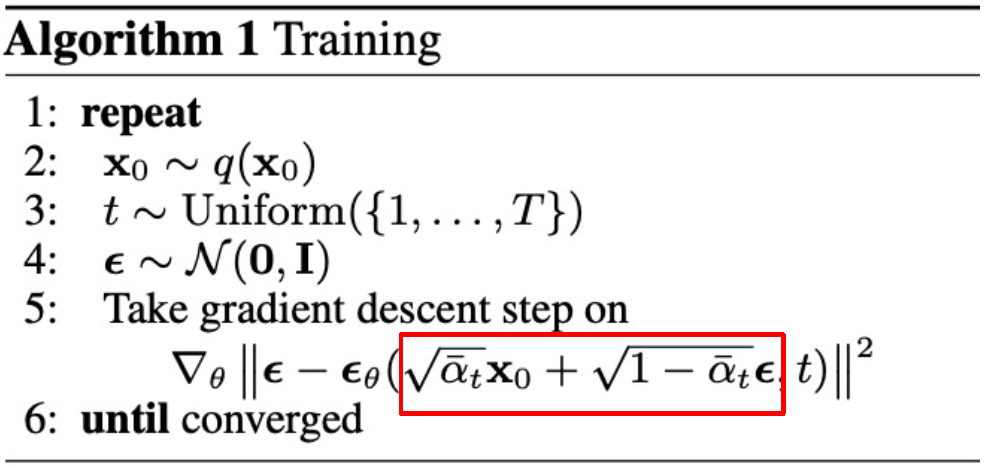
\includegraphics[height=0.7\textheight, width=\textwidth, keepaspectratio]{images/diffusion/diff_5.png}
        \end{figure}
    \end{column}
    \begin{column}{0.5\textwidth}
        \textbf{Training Algorithm}
        \begin{enumerate}
            \item Sample $x_0$ from the data distribution.
            \item Randomly select a timestep $t$.
            \item Corrupt $x_0$ with noise to obtain $x_t$.
            \item Model predicts noise $\epsilon_\theta(x_t, t)$.
            \item Compute loss: mean squared error between predicted and true noise.
            \item Optimize using SGD or Adam.
        \end{enumerate}
    \end{column}
\end{columns}
    
\framebreak

\begin{columns}
    \begin{column}{0.5\textwidth}
        \begin{figure}
            \centering
            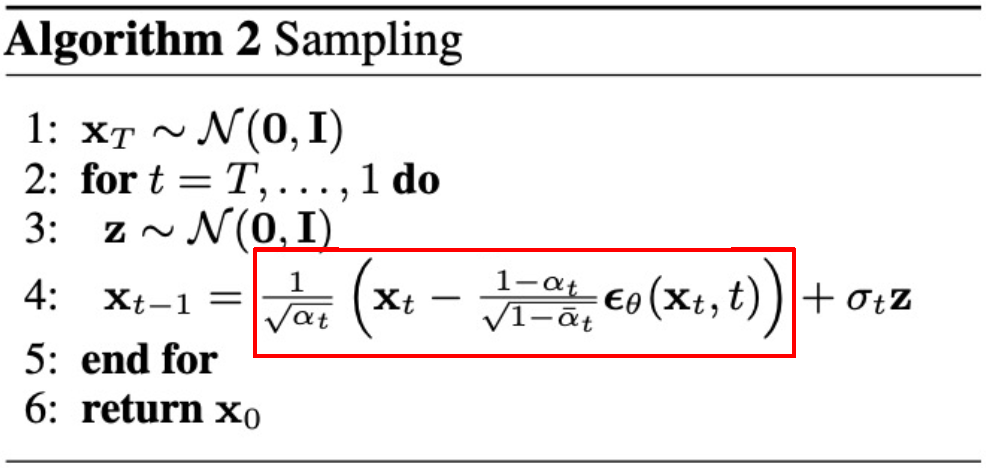
\includegraphics[height=0.7\textheight, width=\textwidth, keepaspectratio]{images/diffusion/diff_6.png}
        \end{figure}
    \end{column}
    \begin{column}{0.5\textwidth}
        \textbf{Sampling Algorithm}
        \begin{enumerate}
            \item Start from Gaussian noise $x_T$.
            \item For each timestep $t = T, \ldots, 1$:
            \begin{enumerate}
                \item Predict noise $\epsilon_\theta(x_t, t)$.
                \item Compute posterior mean $\mu_\theta(x_t, t)$.
                \item Sample $x_{t-1}$ from the Gaussian posterior.
                \item (Optional) Apply guidance (e.g., classifier-free) for improved results.
            \end{enumerate}
        \end{enumerate}
    \end{column}
\end{columns}
    
\end{frame}